\chapter{بازنمایی متن در \eng{TTS}: از \eng{One-Hot} تا بازنمایی وابسته به بافت}

\section{مروری بر معماری سامانه‌های تبدیل متن به گفتار}

در جلسهٔ پیش ساختار کلی سامانه‌های \term{تبدیل متن به گفتار}{Text-to-Speech} را دیدیم. در این جلسه به‌جای تکرار آن مطالب، یک گام عمیق‌تر برمی‌داریم و بخش متنی سامانه را از دید «مدل» و «معماری» بررسی می‌کنیم. سامانه‌های \eng{TTS} را می‌توان به دو شکل کلی ساخت:

\begin{itemize}
  \item \term{معماری خط‌لوله‌ای}{Pipeline-Based}: سامانه از چند ماژول مستقل تشکیل شده و خروجی هر ماژول ورودی ماژول بعدی است.
  \item \term{معماری سرتاسری}{End-to-End}: بخش‌های مختلف پردازش در قالب یک مدل یکپارچه آموخته می‌شوند.
\end{itemize}

تمرکز فعلی درس بر معماری خط‌لوله‌ای است تا بتوانیم هر ماژول را جداگانه بشناسیم و پیاده‌سازی کنیم. مراحل این خط‌لوله در شکل زیر آمده است.

\begin{figure}[htbp]
\centering
\begin{tikzpicture}[rtl, 
  node distance=4mm,
  box/.style={draw, rounded corners=2pt, minimum height=9mm, minimum width=24mm, align=center, font=\small},
  front/.style={box, fill=blue!10},
  back/.style={box, fill=orange!15},
  arr/.style={-{Stealth[length=2.2mm]}, thick}
]
\node[box, fill=gray!10] (txt) {\RL{متن ورودی}\\\lr{Input Text}};
\node[front, below=of txt] (norm) {\RL{نرمال‌سازی متن}\\\lr{Text Normalization}};
\node[front, below=of norm] (homo) {\RL{رفع ابهام هم‌نویسه‌ها}\\\lr{Homograph Disambiguation}};
\node[front, below=of homo] (g2p) {\RL{تولید توالی واج}\\\lr{Phoneme Generation}};
\node[back, right=14mm of g2p] (spec) {\RL{تولید طیف‌نگاشت}\\\lr{Spectrogram Generation}};
\node[back, above=of spec] (wav) {\RL{تولید موج صوتی}\\\lr{Speech Waveform}};
\draw[arr] (txt)--(norm); \draw[arr] (norm)--(homo); \draw[arr] (homo)--(g2p);
\draw[arr] (g2p)--(spec); \draw[arr] (spec)--(wav);
\node[font=\small\bfseries, blue!60!black, left=4mm of homo] {\lr{Front-End}};
\node[font=\small\bfseries, orange!60!black, above=2mm of wav] {\lr{Back-End}};
\end{tikzpicture}
\caption{مراحل معماری خط‌لوله‌ای \eng{TTS}. سه مرحلهٔ آبی «بخش پیشین» و دو مرحلهٔ نارنجی «بخش پسین» سامانه‌اند (شکل افزوده).}
\end{figure}

\begin{definitionbox}{بخش پیشین و بخش پسین}
\term{بخش پیشین}{Front-End} همان بخشی است که با \emph{متن} کار می‌کند: تحلیل و نرمال‌سازی متن، رفع ابهام و استخراج اطلاعات تلفظی. \term{بخش پسین}{Back-End} با بازنمایی‌های \emph{صوتی} سروکار دارد و صدای نهایی را تولید می‌کند. این تقسیم‌بندی مربوط به معماری پردازش گفتار است و نباید با مفاهیم هم‌نام در توسعهٔ وب یکسان گرفته شود.
\end{definitionbox}

\begin{exambox}{تأکید استاد دربارهٔ ماژولار بودن}
هر ماژول را باید جداگانه یاد گرفت؛ زیرا ممکن است در یک پروژه به یکی از آن‌ها بیشتر نیاز داشته باشیم یا بخواهیم چند ماژول را با هم ادغام کنیم. مدل‌های بزرگ سرتاسری ممکن است از نظر منابع محاسباتی و \term{تأخیر}{Latency} محدودیت داشته باشند؛ بنابراین شناخت معماری‌های کوچک‌تر و ماژولار همچنان مهم است. شناخت ماژول‌های مستقل \eng{TTS} پیش از رسیدن به سامانه‌های یکپارچه هدف این مسیر آموزشی است.
\end{exambox}

\textbf{هدف اصلی این جلسه} بررسی بخش متنیِ \eng{TTS}، به‌ویژه تشخیص تلفظ درست \term{هم‌نویسه‌ها}{Homograph} با استفاده از بازنمایی کلمات و اطلاعات بافت جمله است. برای رسیدن به آن، ابتدا باید بدانیم کلمه چگونه به شبکهٔ عصبی داده می‌شود و شبکهٔ عصبی چگونه آموزش می‌بیند.

\section{بازنمایی متن برای شبکه‌های عصبی}

شبکه‌های عصبی مستقیماً با کلمات کار نمی‌کنند؛ آن‌ها به بازنمایی عددی نیاز دارند. پرسشِ «ورودی چگونه نمایش داده می‌شود؟» نخستین پرسش هر مدل زبانی است.

\subsection{بازنمایی \eng{One-Hot}}
ساده‌ترین روش، بردار \term{تک‌داغ}{One-Hot} است. اگر واژگان ما $V$ کلمه داشته باشد، هر کلمه با برداری به طول $V$ نمایش داده می‌شود که فقط یک مؤلفهٔ آن ۱ و بقیه صفر است؛ محل عدد ۱ همان اندیس کلمه در واژگان است. برای واژگانی با پنج کلمه:

\begin{center}
\begin{tabular}{c c}
\toprule
کلمه & بردار \eng{One-Hot} \\
\midrule
کلمهٔ اول & $(1,0,0,0,0)$ \\
کلمهٔ سوم & $(0,0,1,0,0)$ \\
کلمهٔ پنجم & $(0,0,0,0,1)$ \\
\bottomrule
\end{tabular}
\end{center}

این روش با وجود سادگی چهار محدودیت مهم دارد:
\begin{enumerate}
  \item \textbf{ابعاد زیاد:} طول بردار برابر اندازهٔ واژگان است؛ هرچه واژگان بزرگ‌تر شود، حافظهٔ بیشتری لازم است.
  \item \textbf{پراکنده بودن (\eng{Sparse}):} بیشتر مؤلفه‌های هر بردار صفرند.
  \item \textbf{تعامد (\eng{Orthogonality}):} ضرب داخلی هر دو بردار \eng{One-Hot} متعلق به دو کلمهٔ متفاوت صفر است.
  \item \textbf{نبود شباهت معنایی:} مثلاً نام دو شهر یا دو کلمهٔ هم‌معنا در این نمایش هیچ نزدیکی عددی ندارند.
\end{enumerate}

ریشهٔ مشکل این است که کلمات در زبان بر اساس \term{بافت}{Context} و \term{هم‌وقوعی}{Co-occurrence} با یکدیگر مرتبط‌اند، اما \eng{One-Hot} هیچ‌یک از این ارتباطات را نشان نمی‌دهد. برای کاربرد ما، یعنی تشخیص تلفظ از روی بافت، این نقص جدی است.

\subsection{بازنمایی توزیع‌شده: \eng{Word Embedding}}
برای رفع این محدودیت‌ها از \term{تعبیهٔ کلمه}{Word Embedding} استفاده می‌کنیم. به‌جای آنکه طول بردار به اندازهٔ واژگان باشد، یک بُعد دلخواه (مثلاً ۱۲۸ یا ۳۰۰) انتخاب می‌کنیم و به هر کلمه برداری با همین طول نسبت می‌دهیم. هر مؤلفه یک ویژگی عددی است که در فرایند آموزش یاد گرفته می‌شود و لازم نیست از ابتدا مشخص کنیم هر مؤلفه دقیقاً چه چیزی را نشان می‌دهد.

\coursefigure{0.62}{ch08-onehot-vs-dense.png}{مقایسهٔ بردارهای \eng{One-Hot} (پراکنده، با ابعاد زیاد و ازپیش‌تعریف‌شده) و بردارهای \eng{Embedding} (متراکم، با ابعاد کم‌تر و آموخته‌شده از داده). این تصویر در بخش «ورودی چگونه نمایش داده می‌شود؟» تخته آمده بود.}

\begin{table}[htbp]
\centering
\caption{مقایسهٔ دو بازنمایی (جمع‌بندی شکل بالا)}
\begin{tabular}{l c c}
\toprule
ویژگی & \eng{One-Hot} & \eng{Embedding} \\
\midrule
تراکم & پراکنده (\eng{Sparse}) & متراکم (\eng{Dense}) \\
بُعد & برابر اندازهٔ واژگان & کوچک و دلخواه \\
چگونگی ساخت & ازپیش‌تعریف‌شده (\eng{Hard-coded}) & آموخته از داده \\
شباهت معنایی & ندارد & دارد \\
\bottomrule
\end{tabular}
\end{table}

\begin{definitionbox}{بازنمایی توزیع‌شده در برابر پراکنده}
در بازنمایی پراکنده هر کلمه یک «مختصات» منحصربه‌فرد (یک خانهٔ روشن) است. در بازنمایی \term{توزیع‌شده}{Distributed} معنای هر کلمه در چند مؤلفه پخش می‌شود و هر مؤلفه در بازنمایی چندین کلمه نقش دارد؛ به همین دلیل فاصله و زاویهٔ میان بردارها معنا پیدا می‌کند.
\end{definitionbox}

\begin{addedbox}{جدول جست‌وجو و رابطه با \eng{One-Hot}}
اگر $E\in\mathbb{R}^{V\times d}$ ماتریس \eng{Embedding} باشد (هر سطر یک کلمه)، آنگاه ضرب بردار \eng{One-Hot} کلمهٔ $i$ در این ماتریس دقیقاً سطر $i$ام آن را برمی‌گرداند:
\[
\mathbf{e}_i^{\top}E = E_{i,:}.
\]
پس لایهٔ \eng{Embedding} در عمل یک \term{جدول جست‌وجو}{Lookup Table} است و لازم نیست ضرب ماتریسی را واقعاً انجام دهیم. تعداد پارامترهای این لایه $V\times d$ است؛ مثلاً برای $V=50000$ و $d=300$ برابر ۱۵ میلیون عدد.
\end{addedbox}

\begin{addedbox}{مثال عددی: ضرب داخلی و شباهت کسینوسی}
برای دو بردار \eng{One-Hot} متفاوت، همیشه $\mathbf{a}\cdot\mathbf{b}=0$ است؛ پس «گربه» از دید این بازنمایی به «سگ» و «ماشین» به یک اندازه نزدیک است. حال فرض کنید تعبیه‌های دوبُعدیِ فرضیِ زیر را یک مدل یاد گرفته باشد:
\[
\mathbf{v}_{\text{گربه}}=(0.9,\,0.8),\quad
\mathbf{v}_{\text{سگ}}=(0.8,\,0.9),\quad
\mathbf{v}_{\text{ماشین}}=(0.2,\,-0.9).
\]
\term{شباهت کسینوسی}{Cosine Similarity} به‌صورت $\cos\theta=\dfrac{\mathbf{a}\cdot\mathbf{b}}{\|\mathbf{a}\|\,\|\mathbf{b}\|}$ تعریف می‌شود. داریم $\|\mathbf{v}_{\text{گربه}}\|=\|\mathbf{v}_{\text{سگ}}\|=\sqrt{1.45}\approx1.204$ و $\|\mathbf{v}_{\text{ماشین}}\|\approx0.922$. بنابراین
\[
\cos(\text{گربه},\text{سگ})=\frac{0.72+0.72}{1.45}\approx 0.993,
\]
\[
\cos(\text{گربه},\text{ماشین})=\frac{0.18-0.72}{1.204\times0.922}\approx -0.486 .
\]
مقدار نزدیک به $1$ یعنی جهت‌های تقریباً یکسان (کلمات مشابه) و مقدار منفی یعنی جهت‌های مخالف. این همان شباهتی است که \eng{One-Hot} نمی‌تواند نشان دهد.
\end{addedbox}

\coursefigure{0.55}{ch08-cosine-toy.png}{بردارهای فرضیِ مثال بالا در صفحهٔ دوبُعدی؛ زاویهٔ کوچک میان «\eng{cat}» و «\eng{dog}» به شباهت زیاد آن‌ها و زاویهٔ بزرگ نسبت به «\eng{car}» به تفاوت معنایی اشاره دارد (شکل افزوده).}

\subsection{بردارهای \eng{Embedding} چگونه یاد گرفته می‌شوند؟}
بردارها ابتدا به‌صورت تصادفی مقداردهی می‌شوند (\eng{Random Initialization}). سپس باید یک \term{وظیفهٔ آموزشی}{Task} تعریف کنیم. هر شبکه برای یادگیری این چرخه را طی می‌کند:
\begin{enumerate}
  \item ورودی را دریافت می‌کند؛
  \item خروجی را پیش‌بینی می‌کند؛
  \item خروجی را با مقدار صحیح (\eng{Ground Truth}) مقایسه می‌کند؛
  \item خطا را محاسبه می‌کند؛
  \item وزن‌ها را برای کاهش خطا تغییر می‌دهد.
\end{enumerate}
در این میان، بردارهای \eng{Embedding} نیز پارامتر قابل یادگیری‌اند و به‌روز می‌شوند. پس از پایان آموزش می‌توان فقط بردارها را برداشت و در مدل‌های دیگر به کار برد؛ نیازی به نگه‌داشتن کل شبکهٔ آموزش‌دهنده نیست.

\subsubsection{تعریف وظیفه برای یادگیری}
یک وظیفهٔ رایج، پنهان‌کردن بخشی از جمله و خواستن پیش‌بینی آن از مدل است:
\begin{center}
«من امروز به \eng{[MASK]} رفتم.»
\end{center}
مدل باید از روی کلمات اطراف حدس بزند که کلمهٔ حذف‌شده چه بوده است. مزیت مهم این روش آن است که به برچسب‌گذاری دستی نیاز ندارد: متن اصلی را داریم، خودمان یک کلمه را پنهان می‌کنیم و بنابراین پاسخ صحیح از قبل معلوم است. این ویژگی برای مجموعه‌داده‌های متنی بسیار بزرگ حیاتی است (بخش~\ref{sec:selfsup}).

\subsubsection{پیش‌آموزش، تنظیم دقیق و آموزش از صفر}
\begin{itemize}
  \item \term{پیش‌آموزش}{Pre-training}: آموزش مدل روی حجم بزرگی از داده برای یادگیری بازنمایی‌های عمومی زبان.
  \item \term{تنظیم دقیق}{Fine-tuning}: اگر مدل از قبل آموزش دیده باشد، وزن‌های آن را برمی‌داریم و آموزش را با دادهٔ دامنهٔ موردنظر ادامه می‌دهیم تا با نیاز جدید سازگار شود.
  \item \term{آموزش از صفر}{Training from Scratch}: شروع از مقداردهی اولیهٔ جدید و بدون استفاده از وزن‌های ازپیش‌آموخته.
\end{itemize}

اگر دادهٔ ما اصطلاحات تخصصی یا کلمات خارج از واژگان عمومی (\eng{Out-of-Vocabulary} یا \eng{OOV}) داشته باشد، بازنمایی‌های آماده به‌تنهایی کافی نیستند و باید دربارهٔ ادامهٔ آموزش، سازگارسازی با دامنه یا آموزش مدل جدید تصمیم گرفت.

\begin{exambox}{نکتهٔ مورد تأکید استاد}
صرفاً دانلود‌کردن یک \eng{Embedding} آماده همیشه مسئلهٔ یک پروژهٔ تخصصی را حل نمی‌کند. باید بدانیم \eng{Embedding} چگونه ساخته شده و چگونه می‌توان آن را با نیاز خودمان سازگار کرد.
\end{exambox}

\section{مروری بر مبانی شبکه‌های عصبی}

برای فهم چگونگی آموزش \eng{Embedding}ها و مدل‌های تشخیص تلفظ باید اصول شبکه‌های عصبی را مرور کنیم. سطح این مرور مقدماتی است و در پایان جلسه قرار شد همین سطح حفظ شود (بخش~\ref{sec:qa}).

\subsection{ساختار شبکه}
یک شبکهٔ عصبی معمولی از سه بخش ساخته می‌شود:
\begin{itemize}
  \item \term{لایهٔ ورودی}{Input Layer}: دریافت داده، مانند بردار کلمات؛
  \item \term{لایه‌های پنهان}{Hidden Layers}: پردازش و یادگیری بازنمایی‌های میانی؛
  \item \term{لایهٔ خروجی}{Output Layer}: تولید خروجی نهایی، مثل پیش‌بینی یک کلمه یا انتخاب یک کلاس تلفظ.
\end{itemize}

\boardfigure{0.5}{ch08-nn-layers.png}{شبکه‌ای با سه نورون ورودی، دو نورون پنهان و یک نورون خروجی؛ هر یال یک وزن (مانند $w_{1,j}$) دارد.}

با افزایش تعداد لایه‌های پنهان، شبکه «عمیق‌تر» می‌شود و می‌تواند بازنمایی‌های پیچیده‌تر و انتزاعی‌تری بیاموزد. استاد سه وظیفه را از این نظر مقایسه کرد:

\begin{center}
\begin{tabular}{l p{7cm}}
\toprule
وظیفه & ماهیت اطلاعات موردنیاز \\
\midrule
\eng{POS Tagging} & اطلاعات نحوی و نقش کلمات \\
\eng{Named Entity Recognition (NER)} & شناسایی و دسته‌بندی موجودیت‌های نامدار \\
\eng{Commonsense Reasoning} & استدلال بر پایهٔ دانش عمومی و ارتباطات مفهومی \\
\bottomrule
\end{tabular}
\end{center}

\begin{exambox}{قید استاد دربارهٔ مقایسهٔ وظایف}
این ترتیب مطلق نیست. برای مثال \eng{NER} ممکن است فقط چند کلاس رایج داشته باشد یا در یک پروژهٔ تخصصی تعداد بسیار زیادی کلاس و روابط مبتنی بر \eng{Ontology} را شامل شود. عمق موردنیاز شبکه به تعریف دقیق مسئله بستگی دارد.
\end{exambox}

\subsection{نورون: مرحلهٔ پیش‌رو (\eng{Feedforward})}
هر نورون ورودی‌هایش را در وزن‌ها ضرب می‌کند، با هم جمع می‌کند و یک عدد ثابت (بایاس) به آن می‌افزاید. در شکل برداری، برای ورودی $\mathbf{x}$ داریم
\[
\mathbf{z}=W\mathbf{x}+\mathbf{b},\qquad \mathbf{a}=f(\mathbf{z}),
\]
که $W$ ماتریس وزن‌ها، $\mathbf{b}$ بردار بایاس، $\mathbf{z}$ خروجی خطی پیش از تابع فعال‌سازی و $f$ تابع فعال‌سازی است. در شکل تختهٔ کلاس همین رابطه به صورت $y=f(W\cdot x+b)$ نوشته شده بود. وزن‌ها در ابتدا مقدار اولیه می‌گیرند و در آموزش تغییر می‌کنند.

\begin{figure}[htbp]
\centering
\begin{tikzpicture}[
  inp/.style={circle, draw, minimum size=8mm},
  >={Stealth[length=2.2mm]}
]
\node[inp] (x1) at (0,1.8) {$x_1$};
\node[inp] (x2) at (0,0.6) {$x_2$};
\node (xd) at (0,-0.5) {$\vdots$};
\node[inp] (xn) at (0,-1.6) {$x_N$};
\node[circle, draw, minimum size=11mm] (sum) at (4,0.1) {$\Sigma$};
\node[draw, rounded corners=2pt, minimum size=9mm, right=10mm of sum] (act) {$f$};
\node[right=10mm of act] (out) {$a_{\text{\lr{out}}}$};
\node[above=8mm of sum] (b) {$+b$};
\draw[->] (x1)--node[above,pos=.45]{$w_1$}(sum);
\draw[->] (x2)--node[above,pos=.35]{$w_2$}(sum);
\draw[->] (xn)--node[below,pos=.45]{$w_N$}(sum);
\draw[->] (b)--(sum);
\draw[->] (sum)--node[above]{$z$}(act);
\draw[->] (act)--(out);
\end{tikzpicture}
\caption{ساختار یک نورون: جمع وزن‌دار ورودی‌ها به‌علاوهٔ بایاس، $z=b+\sum_i w_ix_i$، و سپس عبور از تابع فعال‌سازی، $a_{\text{\lr{out}}}=f(z)$ (شکل افزوده).}
\end{figure}

\subsubsection{نقش بایاس}
\term{بایاس}{Bias} پارامتر قابل‌یادگیری‌ای است که به مدل اجازه می‌دهد خروجی را مستقل از حاصل‌ضرب وزن‌ها و ورودی جابه‌جا کند. استاد برای شهود از «تخمین کرایهٔ تاکسی» مثال زد: حتی اگر سفر لغو شود (مسافت صفر) هنوز یک هزینهٔ پایه وجود دارد. بایاس همین مقدار پایه را یاد می‌گیرد. اگر بایاس را صفر بگیریم، مدلی «عمومی و بدون هیچ پیش‌فرض» فرض کرده‌ایم، در حالی که در دنیای واقعی پیش‌فرض‌هایی هست که مدل باید یاد بگیرد تا دقیق‌تر تنظیم شود. از نظر هندسی بایاس رابطه را از اجبار عبور از مبدأ آزاد می‌کند.

\subsubsection{تابع فعال‌سازی}
اگر فقط ضرب ماتریسی و جمع بایاس داشته باشیم، ترکیب هر تعداد لایه همچنان یک تبدیل خطی (آفین) است. اما مرزِ بین مفاهیم در دنیای واقعی منحنی، دایره‌ای، پیچ‌درپیچ و چندبُعدی است. \term{تابع فعال‌سازی}{Activation Function} روی خروجی تک‌تک نورون‌ها اعمال می‌شود و رفتار کل شبکه را نسبت به ورودی از یک خط صاف به یک خط شکسته یا منحنی تبدیل می‌کند:
\[
a=f(z).
\]
توابع رایج: \eng{Sigmoid}، \eng{tanh} و \eng{ReLU}. تابع \eng{Sigmoid} و مشتق آن (که در پس‌انتشار لازم می‌شود) چنین است:
\[
\sigma(z)=\frac{1}{1+e^{-z}},\qquad \sigma'(z)=\sigma(z)\bigl(1-\sigma(z)\bigr).
\]

\begin{figure}[htbp]
\centering
\fbox{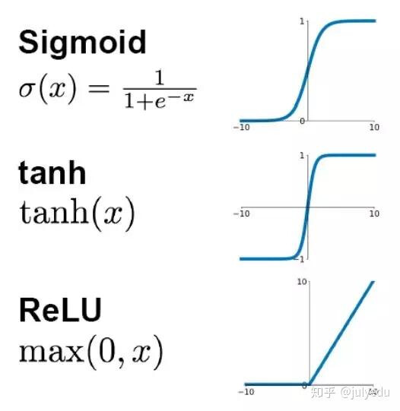
\includegraphics[width=0.45\textwidth]{../assets/figures/ch08-activations.png}}\hfill
\fbox{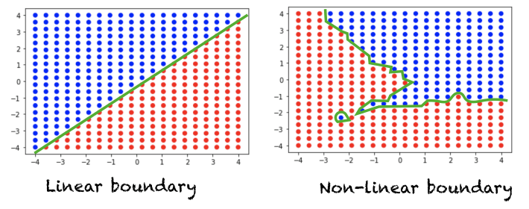
\includegraphics[width=0.45\textwidth]{../assets/figures/ch08-linear-nonlinear.png}}
\caption{سمت راست: توابع \eng{Sigmoid}، \eng{tanh} و \eng{ReLU} با نمودارشان. سمت چپ: مرز تصمیم خطی در برابر مرز غیرخطی؛ تابع فعال‌سازی امکان یادگیری مرزهای غیرخطی را فراهم می‌کند. \textit{(برگرفته از تختهٔ کلاس)}}
\end{figure}

\subsection{خروجی و تابع خطا}
پس از تولید خروجی، آن را با \eng{Ground Truth} مقایسه می‌کنیم. یکی از توابع خطا، \term{میانگین مربعات خطا}{Mean Squared Error}‌ است:
\[
\operatorname{MSE}=\frac{1}{n}\sum_{i=1}^{n}(y_i-\hat{y}_i)^2,
\]
که $n$ تعداد نمونه‌ها یا مؤلفه‌های ارزیابی، $y_i$ مقدار واقعی و $\hat y_i$ مقدار پیش‌بینی‌شده است. هدف آموزش کاهش این مقدار است. (طراحی لایهٔ خروجی و انتخاب تابع خطای مناسب هر نوع مسئله در جلسهٔ بعد تکمیل می‌شود.)

\subsection{چشم‌انداز خطا و کاهش گرادیان}
استاد برای توضیح کاهش خطا از مفهوم \term{چشم‌انداز خطا}{Loss Landscape} استفاده کرد: سطحی که «ارتفاع» آن مقدار خطا و بقیهٔ ابعادش مقادیر وزن‌هاست. با تغییر وزن‌ها، جای ما روی این سطح عوض می‌شود و هدف رسیدن به نواحی با خطای کم‌تر است.

\boardfigure{0.55}{ch08-loss-landscape.png}{چشم‌انداز خطا: محورهای افقی وزن‌ها و محور عمودی مقدار خطاست. از نقطهٔ شروع («\eng{Starting here}») باید به نقطهٔ کمینه («\eng{We want to get to here}») برسیم.}

برای تعیین جهت حرکت، مشتق خطا را نسبت به وزن‌ها محاسبه می‌کنیم. اگر مشتق (شیب) مثبت باشد، یعنی با افزایش وزن خطا زیاد می‌شود؛ پس باید در جهت \emph{مخالف} شیب حرکت کنیم. به بیان استاد: «اگر از لاس مشتق بگیریم و مثبت شد، آن را در منفی ضرب می‌کنیم.» این ایده، مبنای \term{کاهش گرادیان}{Gradient Descent} است.

\begin{figure}[htbp]
\centering
\begin{tikzpicture}[rtl, >=Stealth, line cap=round]
\tikzset{ax/.style={black!60,thin,->}, ln/.style={mainblue,very thick}}
% panel 1: undefined slope (vertical line)
\begin{scope}[shift={(0,0)}]
\draw[ax] (-1.3,0)--(1.3,0); \draw[ax] (0,-1.2)--(0,1.3);
\draw[ln] (0.45,-1.1)--(0.45,1.2);
\node[font=\small] at (0,-1.8) {$m$ تعریف‌نشده};
\end{scope}
% panel 2: zero slope
\begin{scope}[shift={(3.6,0)}]
\draw[ax] (-1.3,0)--(1.3,0); \draw[ax] (0,-1.2)--(0,1.3);
\draw[ln] (-1.1,-0.5)--(1.1,-0.5);
\node[font=\small] at (0,-1.8) {$m=0$};
\end{scope}
% panel 3: negative slope
\begin{scope}[shift={(7.2,0)}]
\draw[ax] (-1.3,0)--(1.3,0); \draw[ax] (0,-1.2)--(0,1.3);
\draw[ln] (-1,0.95)--(1,-0.95);
\node[font=\small] at (0,-1.8) {$m<0$};
\end{scope}
% panel 4: positive slope
\begin{scope}[shift={(10.8,0)}]
\draw[ax] (-1.3,0)--(1.3,0); \draw[ax] (0,-1.2)--(0,1.3);
\draw[ln] (-1,-0.95)--(1,0.95);
\node[font=\small] at (0,-1.8) {$m>0$};
\end{scope}
\end{tikzpicture}
\caption{چهار حالت شیب خط مماس: شیب تعریف‌نشده (خط قائم)، شیب صفر (خط افقی)، شیب منفی و شیب مثبت. علامت شیب جهت لازم برای حرکت به‌سوی کمینه را مشخص می‌کند. (بازسازی‌شده از تختهٔ کلاس)}
\end{figure}

\subsubsection{قاعدهٔ به‌روزرسانی و نرخ یادگیری}
\[
\boxed{\,w_{\text{\lr{new}}}=w_{\text{\lr{old}}}-\eta\,\frac{\partial E}{\partial w}\,}
\]
در این رابطه $\eta$ \term{نرخ یادگیری}{Learning Rate} یا اندازهٔ گام (\eng{step size}) است:
\begin{itemize}
  \item اگر بسیار کوچک باشد، حرکت به‌سوی کمینه کند است؛
  \item اگر مناسب باشد، مدل به‌خوبی همگرا می‌شود؛
  \item اگر بسیار بزرگ باشد، مدل از ناحیهٔ کمینه می‌پرد و ممکن است همگرا نشود.
\end{itemize}
استاد افزود: تا زمانی که واقعیت و تخمین مساوی نشده‌اند، یعنی هنوز چیزی برای یادگیری وجود دارد.

\boardfigure{0.8}{ch08-learning-rate.png}{اثر نرخ یادگیری: بسیار کوچک (گام‌های ریز و کند)، مناسب (رسیدن سریع به کمینه) و بسیار بزرگ (نوسان و واگرایی).}

\begin{addedbox}{مثال عددی: اثر نرخ یادگیری}
تابع ساده $E(w)=w^2$ را با مشتق $E'(w)=2w$ در نظر بگیرید و از $w_0=4$ شروع کنید. قاعدهٔ به‌روزرسانی چنین می‌شود: $w\leftarrow w-\eta\cdot 2w=(1-2\eta)\,w$.
\begin{center}
\begin{tabular}{c c c c c}
\toprule
$\eta$ & $w_0$ & $w_1$ & $w_2$ & رفتار \\
\midrule
$0.1$ & $4$ & $3.2$ & $2.56$ & همگرایی کند \\
$0.5$ & $4$ & $0$ & $0$ & همگرایی یک‌گامی \\
$1.1$ & $4$ & $-4.8$ & $5.76$ & واگرایی (نوسان با دامنهٔ فزاینده) \\
\bottomrule
\end{tabular}
\end{center}
\end{addedbox}

\subsection{پس‌انتشار و قانون زنجیره‌ای}
باید بدانیم هر وزن چه سهمی در خطای خروجی داشته است. این کار با مشتق‌گیری و \term{قانون زنجیره‌ای}{Chain Rule} انجام می‌شود و به آن \term{پس‌انتشار}{Backpropagation} می‌گویند. استاد با شبکه‌ای ساده نشان داد: ورودی، سپس نورون پنهان با خروجی $h$، و سپس نورون خروجی که از طریق وزن $w_5$ به آن وصل است. خروجی خطی و فعال‌شدهٔ آن را چنین می‌گیریم:
\[
\text{net}=h\,w_5+\cdots,\qquad o=\sigma(\text{net}),\qquad E=\tfrac12\,(y-o)^2 .
\]
برای مشتق خطا نسبت به $w_5$ زنجیره را باز می‌کنیم:
\[
\frac{\partial E}{\partial w_5}=\frac{\partial E}{\partial o}\cdot\frac{\partial o}{\partial\,\text{net}}\cdot\frac{\partial\,\text{net}}{\partial w_5}.
\]
سه جزء عبارت‌اند از
\[
\frac{\partial E}{\partial o}=o-y,\qquad
\frac{\partial o}{\partial\,\text{net}}=o(1-o),\qquad
\frac{\partial\,\text{net}}{\partial w_5}=h,
\]
و در نتیجه
\[
\boxed{\;\frac{\partial E}{\partial w_5}=(o-y)\,o\,(1-o)\,h\;}
\]
(در تختهٔ کلاس همین نتیجه به‌صورت $-(y-o)\cdot o(1-o)\cdot h$ نوشته شد.)

\begin{figure}[htbp]
\centering
\begin{tikzpicture}[>=Stealth, font=\small]
\tikzset{unit/.style={circle,draw=mainblue,fill=softblue,minimum size=1.1cm,thick}}
\node[unit] (x) at (0,0) {$x$};
\node[unit] (h) at (3.4,0) {$h$};
\node[unit,minimum size=1.1cm,draw=gray,fill=white,dashed] (h2) at (3.4,-2.1) {$h_2$};
\node[circle,draw=mainblue,fill=softgreen,minimum size=2cm,thick] (o) at (7.2,0) {};
\draw[mainblue,thick] (o.north)--(o.south);
\node at ([xshift=-0.5cm]o.center) {\lr{net}};
\node at ([xshift=0.5cm]o.center) {\lr{out}};
\node[draw=mainblue,fill=softyellow,rounded corners=3pt,inner sep=5pt] (e) at (10.9,0) {$E=\tfrac12\,(y-o)^2$};
\draw[->,thick] (x) -- node[above] {$w_1$} (h);
\draw[->,thick,red!70!black] (h) -- node[above] {$w_5$} (o.west);
\draw[->,dashed,gray] (h2) -- node[below right,pos=0.55,inner sep=1pt] {$w_6$} (o.south west);
\draw[->,thick] (o.east) -- (e.west);
\end{tikzpicture}

\caption{شبکهٔ ساده‌ای که استاد برای پس‌انتشار کشید و محاسبهٔ $\partial E/\partial w_5$ با قانون زنجیره‌ای (روی تخته نورون خروجی با دو بخش «\eng{net}» و «\eng{out}» نمایش داده شده بود). (بازسازی‌شده از تختهٔ کلاس)}
\end{figure}

\boardfigure{0.55}{ch08-chain-rule.png}{بسط قانون زنجیره‌ای روی نمودار یک نورون خروجی (جمع \eng{net}، فعال‌سازی \eng{out} و خطای $\frac12(\text{target}-\text{out})^2$).}

\begin{correctionbox}{دقت در علامت و ضریب مشتق}
در توضیح شفاهی کلاس، علامت و ضریب مشتق خطا به‌دقت تثبیت نشد. نتیجهٔ بالا برای تابع خطای $E=\frac12(y-o)^2$ است؛ ضریب $\frac12$ فقط برای ساده‌شدن مشتق گذاشته می‌شود. اگر تابع خطای دیگری (مثلاً \eng{MSE} با میانگین‌گیری یا \eng{Cross-Entropy}) به کار رود، جزء $\partial E/\partial o$ و ضریب نهایی تغییر می‌کند و باید مطابق تعریف دقیق تابع خطا محاسبه شود.
\end{correctionbox}

\begin{addedbox}{مثال عددی: یک نورون، یک گام پیش‌رو و یک گام یادگیری}
نورونی با دو ورودی $\mathbf{x}=(2,1)$، وزن‌های $\mathbf{w}=(0.4,-0.3)$، بایاس $b=0.1$، تابع فعال‌سازی \eng{Sigmoid} و هدف $y=1$ را در نظر بگیرید.

\textbf{پیش‌رو:} $z=0.4\cdot2+(-0.3)\cdot1+0.1=0.6$ و $o=\sigma(0.6)\approx0.646$. خطا: $E=\frac12(1-0.646)^2\approx0.0628$.

\textbf{پس‌انتشار:} $\delta=(o-y)\,o\,(1-o)=(-0.354)(0.646)(0.354)\approx-0.0811$. پس
\[
\frac{\partial E}{\partial w_1}=\delta\,x_1\approx-0.162,\quad
\frac{\partial E}{\partial w_2}=\delta\,x_2\approx-0.081,\quad
\frac{\partial E}{\partial b}=\delta\approx-0.081 .
\]

\textbf{به‌روزرسانی با $\eta=1$:} $w_1\approx0.562$، $w_2\approx-0.219$ و $b\approx0.181$. اکنون $z\approx1.086$، $o\approx0.748$ و $E\approx0.0318$؛ یعنی خطا تقریباً نصف شد. این چرخهٔ «پیش‌رو، خطا، پس‌انتشار، به‌روزرسانی» بارها تکرار می‌شود.
\end{addedbox}

در مجموع، چرخهٔ آموزش شامل پنج گام است: مقداردهی اولیهٔ تصادفی، \eng{Feedforward}، تولید خروجی، محاسبهٔ \eng{Loss} و در نهایت \eng{Backpropagation} همراه با بهینه‌سازی (به‌روزرسانی وزن‌ها).

\section{مسئلهٔ هم‌نویسه در \eng{TTS}}

اکنون به مسئلهٔ اصلی بازمی‌گردیم: تشخیص تلفظ درست کلماتی که نوشتارشان یکسان است. \term{هم‌نویسه}{Homograph} کلمه‌ای است که شکل نوشتاری یکسان اما تلفظ (و معمولاً معنای) متفاوت دارد. در فارسی چون بیشتر مصوت‌های کوتاه نوشته نمی‌شوند، این مسئله اهمیت ویژه‌ای دارد.

\begin{table}[htbp]
\centering
\caption{نمونه‌های هم‌نویسه در فارسی (آوانویسی تقریبی افزوده شده است)}
\begin{tabular}{c l l}
\toprule
کلمه & بافت اول & بافت دوم \\
\midrule
کرم & کرم مرطوب‌کننده (\eng{kerem}) & کرم خاکی (\eng{kerm}) \\
مرد & آن مرد وارد شد (\eng{mard}) & او از دنیا مرد (\eng{mord}) \\
سرم & سرم به شدت درد می‌کند (\eng{saram}) & سرم را از دستش کشیدند (\eng{serom}) \\
\bottomrule
\end{tabular}
\end{table}

استاد جملهٔ زیر را (که روی تخته نیز بود) نمونه‌ای از وجود چند هم‌نویسه در یک متن می‌دانست: «آن مرد پس از مدت‌ها بیماری در بیمارستان مرد و سرم را از دستش کشیدند. خواهرم گفت: سرم به شدت درد می‌کند.» در این جمله «مرد» دو بار با دو تلفظ و «سرم» دو بار با دو تلفظ و معنا آمده است.

\begin{correctionbox}{«شیر» هم‌نویسهٔ تلفظی نیست}
در کلاس «شیر آب»، «شیر جنگل» و «شیر خوراکی» برای نشان‌دادن مسئله به کار رفت. اما هر سه به یک شکل، یعنی \eng{/ʃir/}، تلفظ می‌شوند؛ «شیر» یک کلمهٔ \emph{چندمعنایی} (هم‌آوا و هم‌نویسه، \eng{Homonym}) است نه هم‌نویسهٔ دارای تلفظ‌های متفاوت. برای \eng{TTS} فقط مواردی مسئله‌ساز است که تلفظ‌ها متفاوت باشند (مانند «کرم» و «مرد»)؛ با این حال «شیر» مثال بسیار خوبی برای نشان‌دادن محدودیت \eng{Embedding} ثابت و نیاز به بافت در فهم \emph{معناست}. در بخش‌های بعد «شیر» را در همین نقش، و «کرم» را برای انتخاب تلفظ به کار می‌بریم.
\end{correctionbox}

\subsection{نقش برچسب‌گذاری نقش دستوری}
گاهی \term{برچسب‌گذاری اجزای کلام}{POS Tagging} برای تشخیص تلفظ کافی است: در «او مُرد» فعل و در «آن مَرد رفت» اسم است و یک برچسب‌زن نحوی با تکیه بر دستور جمله تلفظ درست را مشخص می‌کند. اما همیشه کافی نیست: «کِرم خاکی» و «کِرِم مرطوب‌کننده» هر دو اسم‌اند و برچسب دستوری کمکی نمی‌کند؛ به اطلاعات معنایی و بافتی، یعنی بازنمایی وابسته به بافت (\eng{Contextual Embedding}) نیاز است.

\subsection{چرا \eng{Embedding} برای رفع ابهام مهم است؟}
برای تشخیص تلفظ باید رابطهٔ کلمه با کلمات اطرافش را بدانیم. «کرم خاکی» با واژه‌هایی چون باغچه، خاک و زمین هم‌وقوعی دارد و «کرم مرطوب‌کننده» با پوست، آرایش و محصولات بهداشتی. پس بازنمایی کلمه باید تا حد امکان اطلاعات بافت را در خود داشته باشد؛ این ما را به روش‌های یادگیری \eng{Embedding} بر پایهٔ بافت می‌رساند.

\section{\eng{Embedding} ایستا و \eng{Word2Vec}}

\term{الگوریتم \eng{Word2Vec}}{Word2Vec} بر پایهٔ ارتباط هر کلمه با کلمات اطرافش آموزش می‌بیند و دو معماری اصلی دارد: \eng{CBOW} و \eng{Skip-gram}. بردارهای حاصل \term{ایستا}{Static} هستند: برای هر مدخل واژگان یک بردار ثابت.

\subsection{معماری \eng{CBOW}}
در \term{کیسهٔ کلمات پیوسته}{Continuous Bag of Words} کلمات داخل یک \term{پنجرهٔ بافت}{Context Window} به مدل داده می‌شوند و مدل \emph{کلمهٔ مرکزی} را پیش‌بینی می‌کند. مثلاً از «من، امروز، دانشگاه، رفتم» باید «به» را حدس بزند. در این معماری بازنمایی کلمات اطراف با هم ترکیب (جمع یا میانگین) می‌شوند.

\subsection{معماری \eng{Skip-gram}}
در \eng{Skip-gram} جهت پیش‌بینی برعکس است: کلمهٔ مرکزی ورودی است و مدل \emph{کلمات اطراف} را پیش‌بینی می‌کند؛ مثلاً از «دکتر» باید «مراجعه، کردم، به، امروز» را حدس بزند. به بیان کوتاه: \eng{CBOW}: بافت $\leftarrow$ کلمهٔ هدف؛ \eng{Skip-gram}: کلمهٔ هدف $\leftarrow$ بافت.

\begin{figure}[htbp]
\centering
\begin{tikzpicture}[rtl, >=Stealth, font=\small]
\tikzset{sq/.style={draw=mainblue,fill=softblue,minimum size=0.55cm,inner sep=0pt,thick},
 lab/.style={font=\scriptsize},
 note/.style={draw=mainblue,fill=softyellow,rounded corners=4pt,inner sep=5pt,text width=11.6cm,align=center}}
\node[note] at (5.8,4.7) {\lr{\textbf{Word2Vec}} — \lr{Static Embedding}: یک بردار ثابت برای هر کلمه\\
در زمان آموزش: \lr{Context-Based model}\\ در زمان استنتاج: \lr{Context-independent}};
% headers
\node[lab] at (0,3.1) {\lr{Input}}; \node[lab] at (2.2,3.1) {\lr{Projection}}; \node[lab] at (4.2,3.1) {\lr{Output}};
\node[lab] at (7.4,3.1) {\lr{Input}}; \node[lab] at (9.0,3.1) {\lr{Projection}}; \node[lab] at (11.0,3.1) {\lr{Output}};
% CBOW
\foreach \y/\t [count=\k] in {1.8/{W(t-2)},0.9/{W(t-1)},-0.9/{W(t+1)},-1.8/{W(t+2)}} {
  \node[sq] (c\k) at (0,\y) {}; \node[lab,left=1pt of c\k] {\lr{$\t$}}; }
\node[sq] (cp) at (2.2,0) {}; \node[lab] at (2.2,0.7) {\lr{Sum}};
\node[sq] (co) at (4.2,0) {}; \node[lab,right=1pt of co] {\lr{$W(t)$}};
\foreach \k in {1,2,3,4} \draw[->] (c\k.east) -- (cp.west);
\draw[->] (cp) -- (co);
\node[lab] at (2.2,-2.5) {(a) \lr{CBOW}};
% Skip-gram
\node[sq] (si) at (7.4,0) {}; \node[lab,left=1pt of si] {\lr{$W(t)$}};
\node[sq] (sp) at (9.0,0) {};
\draw[->] (si) -- (sp);
\foreach \y/\t [count=\k] in {1.8/{W(t-2)},0.9/{W(t-1)},-0.9/{W(t+1)},-1.8/{W(t+2)}} {
  \node[sq] (s\k) at (11.0,\y) {}; \node[lab,right=1pt of s\k] {\lr{$\t$}};
  \draw[->] (sp.east) -- (s\k.west); }
\node[lab] at (9.2,-2.5) {(b) \lr{Skip-gram}};
% goals
\node[text width=5cm,align=center,font=\footnotesize] at (1.8,-3.7) {هدف: پیش‌بینی کلمهٔ هدف \lr{(Target)} با استفاده از کلمات پیرامون \lr{(Context)}.};
\node[text width=5cm,align=center,font=\footnotesize] at (9.8,-3.7) {هدف: پیش‌بینی کلمات پیرامون \lr{(Context)} با دریافت یک کلمهٔ ورودی \lr{(Target)}.};
\node[draw=red!70!black,rounded corners=4pt,inner sep=5pt,text width=8cm,align=center,text=red!70!black,font=\footnotesize] at (5.8,-5.3) {برای کاری که کلمات نادر \mbox{\lr{(Rare words)}} زیادی دارد کدام بهتر است؟};
\end{tikzpicture}
\caption{دو معماری \eng{Word2Vec}: \eng{CBOW} و \eng{Skip-gram}، همراه با یادداشت‌های استاد روی تخته. (بازسازی‌شده از تختهٔ کلاس)}
\end{figure}

\begin{correctionbox}{دقت دربارهٔ \eng{CBOW}}
در \eng{CBOW} بازنمایی کلمات پنجره معمولاً \emph{میانگین‌گیری} یا جمع می‌شود (در شکل «\eng{Sum}») و ترتیب کلمات در آن نقشی ندارد؛ از اینجا نام «کیسهٔ کلمات» می‌آید. در نتیجه، همهٔ کلمات اطراف سهم برابر دارند و کلمهٔ بسیار مهم (مثلاً «مریض» برای پیش‌بینی «دکتر» در «من مریض شدم و به دکتر رفتم») نمی‌تواند وزن بیشتری بگیرد. همین نبودِ وزن‌دهی انگیزهٔ مهمی برای سازوکار \eng{Attention} است (بخش~\ref{sec:attention}).
\end{correctionbox}

\subsection{پرسش استاد: برای کلمات نادر کدام بهتر است؟}
پاسخ مورد تأکید: \eng{Skip-gram}. دلیل: در \eng{CBOW} کلمهٔ نادر فقط در جایگاه «هدف» قرار می‌گیرد و چون اطلاعات بافتی چند کلمه در یک بردار ادغام می‌شود، فرصت‌های یادگیری آن کم است. در \eng{Skip-gram} کلمهٔ نادر خودش ورودی است و هر رخداد آن چند جفت آموزشی (کلمه، همسایه) می‌سازد؛ در نتیجه حتی رخدادهای محدود اطلاعاتی دربارهٔ نقش و همسایگی کلمه به مدل می‌دهند. استاد افزود که اگر داده نویز نداشته باشد، حتی یک رخداد نیز ممکن است اطلاعات مفیدی (مثلاً نقش نحوی) بدهد؛ البته یادگیری از نمونهٔ بسیار اندک همچنان محدود است و بازنمایی ممکن است بیش از حد به همان بافت وابسته شود.

\begin{table}[htbp]
\centering
\caption{مقایسهٔ \eng{CBOW} و \eng{Skip-gram}}
\begin{tabular}{l l l}
\toprule
ویژگی & \eng{CBOW} & \eng{Skip-gram} \\
\midrule
ورودی & کلمات اطراف & کلمهٔ مرکزی \\
خروجی & کلمهٔ مرکزی & کلمات اطراف \\
استفاده از بافت & ترکیب اطلاعات کلمات اطراف & پیش‌بینی جداگانهٔ هر کلمهٔ بافت \\
کلمات نادر & دشوارتر یادگرفته می‌شوند & معمولاً مناسب‌تر است \\
نوع \eng{Embedding} نهایی & ایستا & ایستا \\
\bottomrule
\end{tabular}
\end{table}

\subsection{پس از پایان آموزش چه می‌کنیم؟}
هنگام آموزش، وزن‌های شبکه تغییر می‌کنند و بخشی از آن‌ها همان بازنمایی کلمات است. پس از آموزش لازم نیست کل شبکه را نگه داریم: بردارهای \eng{Embedding} را استخراج می‌کنیم و در وظایف دیگر \eng{NLP} (از جمله تشخیص تلفظ) به کار می‌بریم؛ این همان ایدهٔ \eng{Embedding}های ازپیش‌آموزش‌دیده است.

\begin{correctionbox}{چند نکتهٔ فنی دربارهٔ \eng{Word2Vec}}
(۱) \eng{Word2Vec} عملاً دو ماتریس دارد (ماتریس ورودی و ماتریس خروجی)؛ بردار مورد استفاده معمولاً از ماتریس ورودی، یعنی همان «جدول جست‌وجو»، برداشته می‌شود. (۲) در عمل برای کاهش هزینهٔ لایهٔ خروجی با واژگان بزرگ از روش‌هایی مانند \eng{Negative Sampling} یا \eng{Hierarchical Softmax} استفاده می‌شود. (۳) \eng{CBOW} معمولاً سریع‌تر آموزش می‌بیند و برای کلمات پرتکرار خوب است، \eng{Skip-gram} کندتر است ولی برای کلمات نادر بهتر؛ این با توضیح استاد سازگار است.
\end{correctionbox}

\section{گردش کار تشخیص تلفظ در یک سامانهٔ \eng{TTS}}

پس از نرمال‌سازی متن، برای هر کلمه باید معلوم کنیم تلفظش از کجا می‌آید. شکل زیر گردش کاری است که استاد روی تخته ترسیم کرد.

\begin{figure}[htbp]
\centering
\begin{tikzpicture}[rtl, 
  node distance=7mm and 9mm,
  proc/.style={draw, rounded corners=2pt, align=center, minimum height=8mm, text width=30mm, font=\small},
  dec/.style={draw, diamond, aspect=2.2, align=center, inner sep=1pt, font=\small, text width=26mm},
  arr/.style={-{Stealth[length=2.2mm]}, thick},
  lbl/.style={font=\scriptsize, fill=white, inner sep=1pt}
]
\node[proc, fill=gray!10] (w) {\RL{کلمهٔ نرمال‌شده}};
\node[dec, below=of w] (d1) {\RL{آیا کلمه در}\\\RL{واژه‌نامه هست؟}};
\node[dec, below=12mm of d1] (d2) {\RL{آیا هم‌نویسه}\\\RL{است (چند تلفظ)؟}};
\node[proc, left=18mm of d1, fill=orange!15] (oov) {\RL{پردازش کلمهٔ خارج از}\\\RL{واژه‌نامه (\lr{OOV})}};
\node[proc, below=12mm of d2, xshift=-34mm, fill=green!12] (dict) {\RL{استفاده از تلفظ}\\\RL{واژه‌نامه}};
\node[proc, below=12mm of d2, xshift=34mm, fill=blue!10] (dis) {\RL{انتخاب تلفظ با}\\\RL{مدل رفع ابهام}};
\node[proc, below=12mm of $(dict)!0.5!(dis)$, fill=gray!10] (ph) {\RL{توالی واج‌ها}\\\lr{Phonemes}};
\draw[arr] (w)--(d1);
\draw[arr] (d1)--node[lbl,right]{\RL{بله}}(d2);
\draw[arr] (d1)--node[lbl,above]{\RL{خیر}}(oov);
\draw[arr] (d2)-|node[lbl,pos=.15,above=1mm]{\RL{خیر}}(dict);
\draw[arr] (d2)-|node[lbl,pos=.15,above=1mm]{\RL{بله}}(dis);
\draw[arr] (dict)|-(ph);
\draw[arr] (dis)|-(ph);
\draw[arr] (oov)|-(ph);
\end{tikzpicture}
\caption{گردش کار تعیین تلفظ پس از نرمال‌سازی: کلمات واژه‌نامه‌ای با یک تلفظ مستقیماً از واژه‌نامه خوانده می‌شوند، کلمات چندتلفظی به مدل رفع ابهام سپرده می‌شوند و کلمات \eng{OOV} مسیر جداگانه دارند (شکل افزوده، بر پایهٔ تختهٔ کلاس).}
\end{figure}

در این معماری برای کلماتی که چند تلفظ دارند باید مدلی باشد که با نگاه به بافت، تلفظ درست را برگزیند. روش دقیق پردازش \eng{OOV} در این جلسه توضیح داده نشد و تمرکز بر شاخهٔ رفع ابهام هم‌نویسه‌ها بود.

\section{محدودیت \eng{Embedding} ایستا در تشخیص هم‌نویسه}

مهم‌ترین نکتهٔ جلسه تفاوت میان دو چیز است: \eng{Embedding}ای که \emph{در زمان آموزش} بر پایهٔ بافت ساخته شده، و \eng{Embedding}ای که \emph{در زمان استفاده} به بافت جملهٔ جدید وابسته است.

\subsection{مسئله}
فرض کنید کلمهٔ «کرم» در دو جمله آمده: «کرم خاکی در باغچه بود» و «کرم مرطوب‌کننده را روی پوست زدم». در \eng{Word2Vec} برای «کرم» یک بردار ثابت داریم:
\[
E(\text{کرم در جملهٔ اول})=E(\text{کرم در جملهٔ دوم}).
\]
بردار ثابت در زمان آموزش تحت تأثیر همهٔ بافت‌های کلمه ساخته شده است (به‌نوعی «میانگین» آن‌ها)، اما در زمان استفاده برای همهٔ رخدادها یکسان است و دیگر به جملهٔ جدید نگاه نمی‌کند. بنابراین نمی‌توان انتظار داشت بردار ثابت به‌تنهایی تلفظ درست را در هر جمله تعیین کند.

\subsection{راه‌حل با \eng{Embedding} ثابت: افزودن یک مدل انتخاب تلفظ}
استاد پیشنهاد کرد در کنار \eng{Embedding} ثابت یک مدل انتخاب تلفظ بگذاریم:
\begin{enumerate}
  \item \eng{Embedding} ثابت کلمات را داریم؛
  \item کلمات اطراف هم‌نویسه را نیز به مدل می‌دهیم؛
  \item بخش پیش‌بینی‌کننده را با داده‌های دارای برچسب تلفظ آموزش می‌دهیم؛
  \item مدل بر پایهٔ بافت، تلفظ مناسب را انتخاب می‌کند.
\end{enumerate}
یعنی اطلاعات بافت در مدل طبقه‌بند پردازش می‌شود، نه در خود بردار ثابتِ کلمهٔ هدف.

\subsection{استفاده از طبقه‌بند و \eng{Softmax}}
فرض کنید برای کلمه‌ای سه تلفظ ممکن $P_1,P_2,P_3$ در واژه‌نامه باشد. مدل برای هر تلفظ یک امتیاز (\eng{logit}) $\mathbf{z}=(z_1,z_2,z_3)$ می‌دهد و با \eng{Softmax} آن‌ها را به احتمال تبدیل می‌کنیم، که $C$ اطلاعات بافت است:
\[
P(P_i\mid C)=\frac{e^{z_i}}{\sum_j e^{z_j}},\qquad
\hat P=\arg\max_i P(P_i\mid C).
\]
برای نمونه اگر مدل احتمال‌های $0.10$، $0.75$ و $0.15$ را برگرداند، تلفظ دوم انتخاب می‌شود (این اعداد صرفاً برای توضیح سازوکارند).

\begin{addedbox}{مثال عددی: از امتیاز تا احتمال}
فرض کنید امتیازهای مدل برای سه تلفظ $\mathbf{z}=(0.5,\;2.4,\;0.9)$ باشد. آنگاه $e^{z}=(1.65,\;11.02,\;2.46)$، مجموع $\approx15.13$ و
\[
P=(0.109,\;0.728,\;0.163),
\]
که مجموعشان ۱ است و تلفظ دوم برنده است. توجه کنید \eng{Softmax} تفاوت امتیازها را «تیزتر» می‌کند: اختلاف $1.5$ تا $1.9$ واحد در امتیاز، نسبت احتمال را حدود ۷ برابر کرده است.
\end{addedbox}

\subsubsection{داده‌ٔ آموزشی طبقه‌بند}
برای آموزش مدل انتخاب تلفظ باید جملاتی داشته باشیم که تلفظ درست کلمه در آن‌ها مشخص باشد (مثلاً جمله‌ای که «کرم» در آن محصول آرایشی است و جمله‌ای که موجود زنده است). مدل از روی این نمونه‌ها یاد می‌گیرد کدام الگوهای بافتی با کدام تلفظ همراه‌اند و در زمان استنتاج برای جملهٔ جدید یکی از گزینه‌های موجود را برمی‌گزیند.

\subsubsection{اگر تعداد تلفظ‌ها متفاوت باشد؟}
اگر کلمه‌ای دو و کلمهٔ دیگر سه تلفظ داشته باشد، خروجی طبقه‌بند چه شکلی دارد؟ پاسخ استاد: می‌توان در بخش خروجی از یک لایهٔ خطی (\eng{Linear Layer}) و سپس \eng{Softmax} استفاده کرد؛ نکتهٔ مهم این است که مجموعهٔ گزینه‌های تلفظ از پیش مشخص باشد و نگاشت خروجی‌ها به گزینه‌ها با معماری سازگار باشد. معماری دقیق مدیریت تعداد متغیر تلفظ‌ها در این جلسه نهایی نشد و قرار شد در جلسهٔ بعد بررسی شود.

\section{چرا همهٔ تلفظ‌ها را از ابتدا برچسب نمی‌زنیم؟}
\label{sec:selfsup}

یکی از دانشجویان پیشنهاد کرد از همان ابتدا برای هر تلفظ یک بازنمایی جداگانه داشته باشیم (مثلاً «کرم۱»، «کرم۲»، «کرم۳»)؛ در این صورت مدل برای هر یک \eng{Embedding} مجزا یاد می‌گیرد. استاد توضیح داد که از نظر مفهومی ممکن است، اما مشکل اساسی آن است: \emph{چه کسی باید تمام رخدادهای کلمات چندتلفظی را برچسب بزند؟} برای یک مجموعهٔ بزرگ باید مشخص شود هر کلمه در هر جمله کدام تلفظ را دارد؛ در فارسی ممکن است لازم باشد بخش بزرگی از متن اعراب‌گذاری یا تلفظ کلمات مبهم دستی تعیین شود. این فرایند بسیار پرهزینه است.

\begin{exambox}{تأکید استاد}
\term{برچسب‌گذاری}{Annotation} یکی از گلوگاه‌های مهم توسعهٔ سامانه‌های هوش مصنوعی است.
\end{exambox}

\subsection{راه‌حل: وظایفی که برچسب خودکار دارند}
یکی از دلایل موفقیت مدل‌های زبانی بزرگ این بود که توانستند از حجم عظیمی از متن بی‌برچسب استفاده کنند. به‌جای اینکه انسان برای هر جمله برچسب تهیه کند، وظیفه‌ای تعریف می‌کنیم که پاسخش از خود متن به‌دست می‌آید:
\begin{itemize}
  \item \term{مدل‌سازی زبان نقاب‌دار}{Masked Language Modeling} (\eng{MLM}): برخی کلمات پنهان می‌شوند و مدل باید آن‌ها را پیش‌بینی کند؛
  \item \term{پیش‌بینی جملهٔ بعدی}{Next Sentence Prediction} (\eng{NSP}): در مدل اولیهٔ \eng{BERT}، مدل یاد می‌گیرد آیا یک جمله ادامهٔ جملهٔ دیگری است یا نه.
\end{itemize}
برای ساخت دادهٔ این وظایف، نیازی به تعیین دستی تلفظ همهٔ کلمات نیست؛ مدل از ساختار و روابط خود متن یاد می‌گیرد.

\begin{correctionbox}{دقت دربارهٔ \eng{NSP}}
\eng{NSP} در مقالهٔ اولیهٔ \eng{BERT} به کار رفت، اما در پژوهش‌های بعدی (مانند \eng{RoBERTa}) نشان داده شد که حذف آن آسیبی به کیفیت نمی‌زند و بسیاری از مدل‌های جدید فقط از شکلی از \eng{MLM} یا پیش‌بینی توکن بعدی استفاده می‌کنند. بنابراین \eng{MLM} را باید وظیفهٔ اصلی و \eng{NSP} را یک نمونهٔ تاریخی دانست. جزئیات \eng{BERT} در جلسهٔ بعد می‌آید.
\end{correctionbox}

\subsection{یادگیری خودنظارتی}
این نوع آموزش در چارچوب \term{یادگیری خودنظارتی}{Self-Supervised Learning} قرار می‌گیرد: سیگنال آموزشی از خود داده استخراج می‌شود. نتیجه:
\begin{itemize}
  \item نیاز به برچسب‌گذاری دستی کاهش می‌یابد؛
  \item استفاده از داده‌های متنی بسیار بزرگ ممکن می‌شود؛
  \item مدل بازنمایی‌های عمومی زبان را می‌آموزد؛
  \item بعداً می‌توان آن را برای وظایف تخصصی تنظیم دقیق کرد.
\end{itemize}
\begin{definitionbox}{یادگیری نظارتی در برابر خودنظارتی}
در \term{یادگیری نظارتی}{Supervised Learning} انسان داده را برچسب می‌زند (مثلاً جمله را «مثبت» یا «منفی» می‌کند). در یادگیری خودنظارتی برچسب از خود داده ساخته می‌شود، مثلاً کلمهٔ حذف‌شده از متن اصلی. استاد تأکید کرد یکی از جهش‌های بزرگ مدل‌های زبانی همین استفاده از داده‌های عظیم و وظایف قابل‌استخراج از خود متن بود.
\end{definitionbox}

\section{\eng{Embedding} وابسته به بافت (پویا)}

پس از دیدن محدودیت \eng{Embedding} ایستا، پرسش این است: چگونه \eng{Embedding} را طوری بسازیم که برای هر جمله و بر پایهٔ بافت همان جمله تغییر کند؟ پاسخ، \term{\eng{Embedding} وابسته به بافت}{Contextual Embedding} (یا پویا، \eng{Dynamic}) است.

\subsection{مقایسهٔ ایستا و وابسته به بافت}
در بازنمایی ایستا
\[
E(w)=\mathbf{v}_w,
\]
بردار فقط به هویت کلمه بستگی دارد. در بازنمایی وابسته به بافت
\[
E(w,C)=\mathbf{v}_{w,C},
\]
که $C$ جملهٔ حاوی کلمه است، و ممکن است $E(\text{کرم},C_1)\neq E(\text{کرم},C_2)$.

\begin{figure}[htbp]
\centering
\begin{tikzpicture}[rtl, >=Stealth, font=\footnotesize]
\tikzset{bx/.style={draw=mainblue,fill=softgreen,rounded corners=6pt,thick,inner sep=6pt,text width=6.4cm,align=center},
 ov/.style={draw=mainblue,fill=softyellow,rounded corners=14pt,thick,inner sep=7pt,text width=5.6cm,align=center}}
\node[diamond,draw=mainblue,fill=softgreen,thick,aspect=2.2,inner sep=3pt,font=\small] (top) at (0,0) {لایهٔ امبدینگ};
\node[bx,anchor=north] (st) at (-3.7,-1.7) {\textbf{امبدینگ ایستا \lr{(Static)}}\\[3pt]
هر روشی که طی آن بردار خروجی یک کلمه تابعی از تمامی جملاتی باشد که در زمان آموزش، آن کلمه در بافت آن‌ها ظاهر شده است.\\[3pt]
\textbf{در زمان استفاده:} کلمه به‌تنهایی و بدون دیدن کل جمله وارد یک جدول جست‌وجو \lr{(Lookup Table)} می‌شود.\\[3pt]
\textbf{چیزی که دانلود می‌کنید:} یک فایل که در آن مثلاً کلمهٔ «شیر» یک سطر با ۳۰۰ عدد مشخص دارد و فرقی نمی‌کند منظور «شیر جنگل»، «شیر آب» یا «شیر خوراکی» باشد؛ بردار همیشه ثابت است و بدون نیاز به شبکهٔ عصبی مستقیماً از حافظه خوانده می‌شود.};
\node[bx,anchor=north] (dy) at (3.7,-1.7) {\textbf{امبدینگ داینامیک / \lr{Contextual}}\\[3pt]
هر روشی که طی آن بردار خروجی یک کلمه، تابعی از کل کلمات موجود در جملهٔ فعلی باشد.\\[3pt]
\textbf{در زمان استفاده:} کلمه در بستر کل جمله وارد شبکه می‌شود. شبکه کل جمله را پردازش می‌کند و بر اساس رابطهٔ آن کلمه با همسایه‌هایش، بردار نهایی را می‌سازد.\\[3pt]
\textbf{چیزی که دانلود می‌کنید:} وزن‌های شبکه \lr{(Weights \& Biases)}. بردار کلمه وجود خارجی ندارد تا زمانی که جمله وارد شبکه شود.};
\draw[->,thick] (top.south west) -- ++(-0.6,-0.1) -| (st.north);
\draw[->,thick] (top.south east) -- ++(0.6,-0.1) -| (dy.north);
\node[ov,anchor=north] (sa) at (-3.7,-10.3) {\lr{\textbf{Self-Attention}}\\[3pt]
نمایش تمام موقعیت‌های ورودی را در اختیار داشته باش.\\
ارتباط هر موقعیت را با موقعیت‌های دیگر محاسبه کن.\\
بر اساس وزن‌های ارتباط، اطلاعات موقعیت‌ها را ترکیب کن تا نمایش جدید هر موقعیت به دست آید.};
\node[ov,anchor=north] (ls) at (3.7,-10.3) {\lr{\textbf{LSTM}}\\[3pt]
ورودی‌ها را به‌ترتیب پردازش کن.\\
اطلاعات هر گام را از طریق حالت بازگشتی به گام بعد منتقل کن.};
\draw[->,thick] (dy.south) -- (3.7,-9.6) -| (sa.north);
\draw[->,thick] (dy.south) -- (3.7,-9.6) -| (ls.north);
\end{tikzpicture}
\caption{دو نوع لایهٔ \eng{Embedding}. چپ: \eng{Embedding} ایستا (بردار تابعی از همهٔ جمله‌هایی است که کلمه در زمان آموزش در آن‌ها دیده شده؛ در زمان استفاده فقط یک جدول جست‌وجو). راست: \eng{Embedding} پویا (بردار تابعی از کل کلمات جملهٔ فعلی است؛ چیزی که دانلود می‌کنید وزن‌های شبکه است). دو بیضی پایین دو راه ساخت آن را نشان می‌دهند: \eng{Self-Attention} و \eng{LSTM}. (بازسازی‌شده از تختهٔ کلاس)}
\end{figure}

\begin{table}[htbp]
\centering
\caption{مقایسهٔ دو نوع \eng{Embedding} به روایت تختهٔ کلاس}
\begin{tabular}{p{3cm} p{5.5cm} p{5.5cm}}
\toprule
 & ایستا & وابسته به بافت \\
\midrule
تعریف & بردار خروجی تابعی از همهٔ جمله‌هایی است که کلمه در زمان آموزش در بافتشان دیده شده & بردار خروجی تابعی از کل کلمات جملهٔ فعلی است \\
زمان استفاده & کلمه به‌تنهایی وارد جدول جست‌وجو می‌شود & کلمه در بستر جمله وارد شبکه می‌شود و شبکه بر پایهٔ رابطه با همسایه‌ها بردار نهایی را می‌سازد \\
چیزی که دانلود می‌کنید & فایلی که به‌ازای هر کلمه یک سطر (مثلاً ۳۰۰ عدد) دارد؛ «شیر» در هر معنایی همان بردار است و مستقیماً از حافظه خوانده می‌شود & وزن‌های شبکه (\eng{Weights \& Biases})؛ بردار کلمه تا ورود جمله به شبکه وجود خارجی ندارد \\
\bottomrule
\end{tabular}
\end{table}

\subsection{هدف}
مدل هنگام دریافت یک جمله باید: (۱) کلمات جمله را دریافت کند، (۲) برای ساخت بازنمایی هر کلمه سایر کلمات را در نظر بگیرد، (۳) اهمیت ارتباط هر کلمه با بقیه را بسنجد و (۴) بازنمایی متناسب با همین رخداد را بسازد. مثلاً برای «کرم» در یک جمله «خاک» و «باغچه» مهم‌اند و در جملهٔ دیگر «پوست» و «مرطوب‌کننده».

\section{استفاده از \eng{Attention} برای ساخت \eng{Embedding} وابسته به بافت}
\label{sec:attention}

یکی از راه‌های مهم ساخت بازنمایی وابسته به بافت، \term{سازوکار توجه}{Attention Mechanism} است. تختهٔ کلاس سه گام آن را چنین خلاصه کرد: (۱) نمایش همهٔ موقعیت‌های ورودی را در اختیار داشته باش؛ (۲) ارتباط هر موقعیت را با موقعیت‌های دیگر محاسبه کن؛ (۳) بر اساس وزن‌های ارتباط، اطلاعات موقعیت‌ها را ترکیب کن تا نمایش جدید هر موقعیت به‌دست آید. (راه دیگر ساخت بازنمایی پویا، پردازش ترتیبی با \eng{LSTM} است که در تخته آمد و در جلسهٔ بعد بیشتر می‌آید.)

\subsection{ایدهٔ اصلی}
به‌جای ترکیب یکسان همهٔ کلمات اطراف (مانند \eng{CBOW}) مدل مشخص می‌کند هر کلمه چقدر به کلمهٔ موردنظر مرتبط است. مثلاً در جمله‌ای دربارهٔ «کرم خاکی»، ارتباط «کرم» با «خاک» می‌تواند بیش از ارتباط آن با یک کلمهٔ کم‌اهمیت باشد.

\subsection{مفاهیم \eng{Query}، \eng{Key} و \eng{Value}}
\begin{itemize}
  \item \term{پرس‌وجو}{Query} ($Q$): نمایندهٔ چیزی که برایش اطلاعات مرتبط می‌جوییم (کلمهٔ هدف).
  \item \term{کلید}{Key} ($K$): برای سنجش میزان ارتباط هر کلمه با پرس‌وجو به کار می‌رود.
  \item \term{مقدار}{Value} ($V$): اطلاعاتی که با توجه به میزان ارتباط در ساخت خروجی شرکت می‌کند.
\end{itemize}
کلمهٔ هدف به‌عنوان \eng{Query} با \eng{Key} کلمات جمله مقایسه می‌شود؛ شباهت \eng{Query} و \eng{Key} میزان توجه به هر کلمه را می‌دهد و سپس \eng{Value}ها با این وزن‌ها ترکیب می‌شوند تا بازنمایی جدید ساخته شود. ماتریس‌های وزنی \eng{Q}، \eng{K} و \eng{V} در آموزش یاد گرفته می‌شوند و در زمان استنتاج ثابت‌اند؛ آنچه با جمله عوض می‌شود بردارهای \eng{Q}، \eng{K} و \eng{V} محاسبه‌شده و در نتیجه بازنمایی خروجی است.

\subsection{نقش ضرب داخلی و فرمول کامل}
برای سنجش ارتباط \eng{Query} و \eng{Key} از ضرب داخلی استفاده می‌شود: امتیاز $Q\cdot K$ هرچه بزرگ‌تر، سهم آن کلمه بیشتر. استاد تصریح کرد که \eng{Attention} فقط یک ضرب ساده نیست و در این جلسه هدف درک شهودی بود. فرمول کامل \term{توجه ضرب داخلیِ مقیاس‌شده}{Scaled Dot-Product Attention} چنین است:
\[
\operatorname{Attention}(Q,K,V)=\operatorname{softmax}\!\left(\frac{QK^{\top}}{\sqrt{d_k}}\right)V ,
\]
که $d_k$ بُعد بردارهای \eng{Key} است. تقسیم بر $\sqrt{d_k}$ از بزرگ‌شدن بیش از حد امتیازها در بُعد زیاد (و اشباع \eng{Softmax}) جلوگیری می‌کند. \eng{Softmax} امتیازهای هر سطر را به وزن‌های نامنفی با مجموع ۱ تبدیل می‌کند و ضرب در $V$ ترکیب وزن‌دار مقدارها را می‌دهد.

\begin{addedbox}{مثال عددی: \eng{Self-Attention} با دو توکن}
جملهٔ بسیار کوتاه «کرم خاک» را با دو توکن در نظر بگیرید و برای سادگی $X=\begin{pmatrix}1&0\\0&1\end{pmatrix}$ (سطر اول «کرم»، سطر دوم «خاک»). فرض کنید ماتریس‌های آموخته‌شده چنین باشند:
\[
W_Q=\begin{pmatrix}1&1\\0&2\end{pmatrix},\quad
W_K=\begin{pmatrix}2&0\\0&1\end{pmatrix},\quad
W_V=\begin{pmatrix}1&0\\1&1\end{pmatrix}.
\]
آنگاه
\[
Q=XW_Q=\begin{pmatrix}1&1\\0&2\end{pmatrix},\quad
K=XW_K=\begin{pmatrix}2&0\\0&1\end{pmatrix},\quad
V=XW_V=\begin{pmatrix}1&0\\1&1\end{pmatrix}.
\]
امتیازها پیش و پس از تقسیم بر $\sqrt{2}\approx1.414$ چنین‌اند:
\[
QK^{\top}=\begin{pmatrix}2&1\\0&2\end{pmatrix}
\;\longrightarrow\;
\frac{QK^{\top}}{\sqrt2}=\begin{pmatrix}1.414&0.707\\0&1.414\end{pmatrix}.
\]

\eng{Softmax} روی هر سطر: در سطر اول $e^{1.414}\approx4.11$ و $e^{0.707}\approx2.03$ است، پس وزن‌ها $\frac{4.11}{6.14}\approx0.670$ و $0.330$ می‌شوند؛ در سطر دوم $e^{0}=1$ و $e^{1.414}\approx4.11$ و وزن‌ها $0.196$ و $0.804$ است. پس
\[
A=\begin{pmatrix}0.670&0.330\\0.196&0.804\end{pmatrix},\qquad
AV=\begin{pmatrix}0.670\cdot(1,0)+0.330\cdot(1,1)\\ 0.196\cdot(1,0)+0.804\cdot(1,1)\end{pmatrix}
=\begin{pmatrix}1.00&0.33\\1.00&0.80\end{pmatrix}.
\]
بازنمایی جدید «کرم» سطر اول $AV$ است: ترکیبی با ۶۷٪ سهم از مقدار خودش و ۳۳٪ سهم از مقدار «خاک». اگر در جملهٔ دیگری کنار «کرم» توکنی مانند «پوست» بود، وزن‌های $A$ و در نتیجه بردار خروجی متفاوت می‌شد؛ همین یعنی بازنمایی «وابسته به بافت».
\end{addedbox}

\subsection{\eng{Self-Attention}}
وقتی کلمات یک توالی برای ساخت بازنمایی جدید خودشان به کلمات همان توالی توجه می‌کنند، از \term{خودتوجهی}{Self-Attention} صحبت می‌کنیم. اگر «کرم» در جمله‌ای با «خاکی» و «باغچه» بیاید، بازنمایی متناسب با موجود زنده ساخته می‌شود و اگر کنار «پوست» و «مرطوب‌کننده» بیاید، بازنمایی دیگری. به این ترتیب بخشی از مشکل \eng{Embedding} ایستا برطرف می‌شود.

\subsection{ارتباط با \eng{Transformer}}
\eng{Self-Attention} از اجزای اصلی معماری \term{ترنسفورمر}{Transformer} است که در ادامهٔ درس به آن می‌رسیم؛ این سازوکار به مدل کمک می‌کند برای هر توکن، اطلاعات سایر توکن‌های جمله را در نظر بگیرد. تفاوت اصلی از نگاه استاد: در \eng{Word2Vec} بردار نهایی کلمه پس از آموزش ثابت است، اما در مدل مبتنی بر \eng{Self-Attention} شبکه در زمان استنتاج نیز با هر جملهٔ جدید اجرا می‌شود و بازنمایی همان جمله را حساب می‌کند.

\begin{correctionbox}{دقت دربارهٔ «بردار ثابت» و «بردار پویا»}
بازنمایی وابسته به بافت به این معنا نیست که وزن‌های شبکه در استنتاج عوض می‌شوند؛ وزن‌ها ثابت‌اند و فقط \emph{خروجی} به‌ازای جملهٔ ورودی متفاوت است. همچنین \eng{Contextual Embedding} با \eng{Transformer} یکی نیست: \eng{LSTM} دوسویه (مانند \eng{ELMo}) نیز بازنمایی وابسته به بافت می‌سازد؛ \eng{Attention} یکی از راه‌هاست.
\end{correctionbox}

\section{پرسش و پاسخ پایان کلاس}
\label{sec:qa}

\begin{itemize}
  \item \textbf{بخش پیشین (\eng{Front-End}) در \eng{TTS} دقیقاً چیست؟}\\ ماژول‌هایی که روی متنِ ورودی کاربر عمل می‌کنند؛ در مقابل، بخش پسین به بازنمایی‌های صوتی و تولید گفتار مربوط است و با مفاهیم هم‌نام در توسعهٔ وب یکی نیست.
  \item \textbf{آیا با \eng{Embedding} ایستا می‌توان تلفظ هم‌نویسه را تشخیص داد؟}\\ بله، اما بردار ثابت یک کلمه کافی نیست؛ باید اطلاعات کلمات اطراف نیز به یک مدل پیش‌بینی داده شود که با داده‌های برچسب‌دار یاد بگیرد در هر بافت کدام تلفظ مناسب است.
  \item \textbf{آیا بهتر نیست برای هر تلفظ از ابتدا \eng{Embedding} مجزا بسازیم؟}\\ از نظر طراحی می‌شود، ولی به داده‌های برچسب‌خورده و برچسب‌گذاری گستردهٔ پرهزینه نیاز دارد؛ از این رو پیش‌آموزش با یادگیری خودنظارتی اهمیت دارد.
  \item \textbf{طبقه‌بند چگونه تلفظ درست را می‌گزیند؟}\\ در خروجی برای هر گزینه امتیاز تولید می‌کند، با \eng{Linear Layer} و \eng{Softmax} احتمال را می‌سنجد و تلفظ با بیشترین احتمال را برمی‌گزیند؛ یادگیری این تصمیم نیازمند نمونه‌هایی از کلمه در بافت‌های مختلف همراه با تلفظ صحیح است.
  \item \textbf{آیا مباحث شبکهٔ عصبی باید با جزئیات بیشتری تدریس شوند؟}\\ استاد از دانشجویان پرسید؛ به موضوعاتی مانند \term{مومنتوم}{Momentum} (بهینه‌سازی با «حافظهٔ» گام‌های قبلی) اشاره شد و قرار شد فعلاً همین سطح مقدماتی حفظ شود.
\end{itemize}

\section{آنچه در جلسهٔ بعد ادامه می‌یابد}

استاد اعلام کرد در جلسهٔ بعد تصمیم‌گیری نهایی مدل انتخاب تلفظ با جزئیات بیشتر بررسی می‌شود. موضوعات اعلام‌شده:
\begin{itemize}
  \item بررسی دقیق‌تر لایهٔ خروجی برای انتخاب تلفظ؛
  \item نحوهٔ تصمیم‌گیری مدل با امتیازهای خروجی و \eng{Softmax}؛
  \item ادامهٔ معماری‌های مبتنی بر بافت؛
  \item ورود تدریجی به \eng{Transformer} و سپس معماری‌های سرتاسری.
\end{itemize}

\section{جمع‌بندی}

مسیر مفهومی این جلسه از بازنمایی عددی ساده تا بازنمایی وابسته به بافت بود. کلمه ابتدا با \eng{One-Hot} نمایش داده می‌شود که پراکنده است و شباهت معنایی ندارد. \eng{Embedding} متراکم و آموخته‌شده این کمبود را جبران می‌کند، و \eng{Word2Vec} (\eng{CBOW} و \eng{Skip-gram}) آن را از روی هم‌وقوعی کلمات می‌سازد. اما بردار \eng{Word2Vec} ایستاست و برای کلمه‌ای مانند «کرم» در همهٔ جمله‌ها یکسان می‌ماند؛ بنابراین برای \eng{TTS} باید یا مدلی روی بافت بگذاریم و با داده‌های برچسب‌دار آموزشش دهیم، یا (راه بنیادی‌تر) از بازنمایی وابسته به بافت بهره بگیریم. چون برچسب‌گذاری دستی گران است، پیش‌آموزش خودنظارتی (مانند \eng{MLM}) اهمیت می‌یابد و \eng{Self-Attention} ابزار اصلی ساخت این بازنمایی‌هاست.

\begin{table}[htbp]
\centering
\caption{جدول مفاهیم کلیدی جلسه}
\begin{tabular}{l p{9cm}}
\toprule
مفهوم & نکتهٔ اصلی \\
\midrule
\eng{One-Hot} & ساده، پراکنده و فاقد شباهت کلمات \\
\eng{Word Embedding} & بازنمایی عددی متراکم و آموخته‌شدهٔ کلمات \\
\eng{Feedforward} & محاسبهٔ خروجی با وزن‌ها، بایاس و فعال‌سازی \\
\eng{Backpropagation} & محاسبهٔ گرادیان خطا نسبت به پارامترها با قانون زنجیره‌ای \\
\eng{Gradient Descent} & تغییر وزن‌ها در خلاف جهت گرادیان با گام $\eta$ \\
\eng{CBOW} / \eng{Skip-gram} & پیش‌بینی هدف از بافت / پیش‌بینی بافت از هدف؛ \eng{Skip-gram} برای کلمات نادر بهتر \\
\eng{Homograph} & نوشتار یکسان با تلفظ و معنای متفاوت \\
\eng{Static Embedding} & بردار ثابت برای هر کلمه در زمان استنتاج \\
\eng{Contextual Embedding} & بردار هر کلمه تابعی از جملهٔ فعلی \\
\eng{Self-Attention} & ساخت بازنمایی وابسته به بافت با $\operatorname{softmax}(QK^{\top}/\sqrt{d_k})V$ \\
\bottomrule
\end{tabular}
\end{table}

\begin{exambox}{نکات مهم برای مرور و امتحان}
\begin{itemize}
  \item تفاوت \eng{Pipeline} و \eng{End-to-End}؛ تعریف \eng{Front-End} و \eng{Back-End}.
  \item چهار محدودیت \eng{One-Hot} و مزایای \eng{Embedding} (تراکم، بُعد کم، شباهت معنایی، آموخته از داده).
  \item چرخهٔ آموزش شبکه: مقداردهی تصادفی، \eng{Feedforward}، خروجی، \eng{Loss}، \eng{Backpropagation} و به‌روزرسانی؛ رابطهٔ $w_{\text{\lr{new}}}=w_{\text{\lr{old}}}-\eta\,\partial E/\partial w$ و اثر نرخ یادگیری.
  \item نقش بایاس (مثال کرایهٔ تاکسی) و تابع فعال‌سازی (غیرخطی‌کردن).
  \item تفاوت \eng{CBOW} و \eng{Skip-gram} و اینکه برای کلمات نادر \eng{Skip-gram} بهتر است.
  \item \eng{Embedding} ایستا: در آموزش وابسته به بافت، در استنتاج مستقل از بافت؛ چرا برای هم‌نویسه کافی نیست.
  \item چرا همهٔ تلفظ‌ها را از ابتدا برچسب نمی‌زنیم (گلوگاه \eng{Annotation}) و نقش \eng{Self-Supervised Learning}.
  \item مفاهیم \eng{Query}/\eng{Key}/\eng{Value} و فرمول \eng{Attention}.
\end{itemize}
\end{exambox}
